\chapter{Modulador 16-QAM}
\label{section:qam}


En este capítulo se muestra el bloque encargado de la modulación 16-QAM. Este bloque se compone de tres procesos: mapeado 16-QAM, aplicación de Zero Padding y filtrado Root Raise Cosine. En la Figura \ref{fig:qam_fir} se puede visualizar la estructura de los bloques IP que se han incluido en este segundo proyecto de Vivado. 

\vspace{2mm}

\begin{figure}[h]
	\centering
	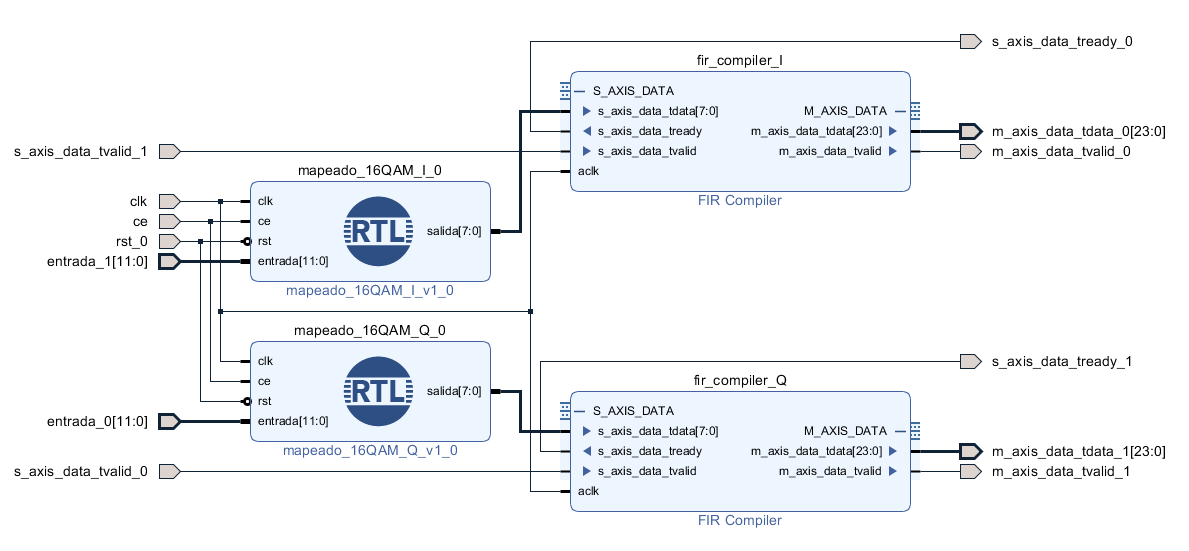
\includegraphics[width=1\textwidth]{img/diseno/qam_fir.PNG}
	\caption{Diseño de los bloques mapeado 16-QAM + ZP y filtrado RRC}
	\label{fig:qam_fir}
\end{figure}
    
\vspace{1mm}

\section{Mapeado 16-QAM}

Para implementar una modulación 16-QAM (Modulación de Amplitud en Cuadratura) lo primero que se debe realizar es el bloque de mapeado, con el fin de asignar patrones de amplitud y fase a cada símbolo y proporcionar una mayor eficiencia espectral. Para ello, se recibe una señal de entrada de 12 bits, obtenida a partir de la lectura de los 200 valores almacenados en la memoria FIFO. 

\pagebreak

Como se había descrito en el Capítulo \ref{section:xadc_fifo}, la lectura se produce a una frecuencia de 2MHz. Según las especificaciones de este proyecto, la salida del mapeado debe funcionar a una frecuencia de 6MHz, es decir, el triple de la anterior porque por cada valor a la entrada de 12 bits se obtendrán 3 símbolos 16-QAM. En otros términos, se tratarán los bits de entrada de 4 en 4 para mapear cada símbolo 16-QAM. 

El mapeado de cada símbolo 16-QAM supone la generación a la salida de dos caminos independientes: uno para la componente en Fase (I) y otro para la de Cuadratura (Q). Cada símbolo es de 3 bits con signo y puede tomar los valores (-3,-1,+1,+3) como se puede visualizar en la Figura \ref{fig:qam}.

\vspace{3mm}

\begin{figure}[h]
	\centering
	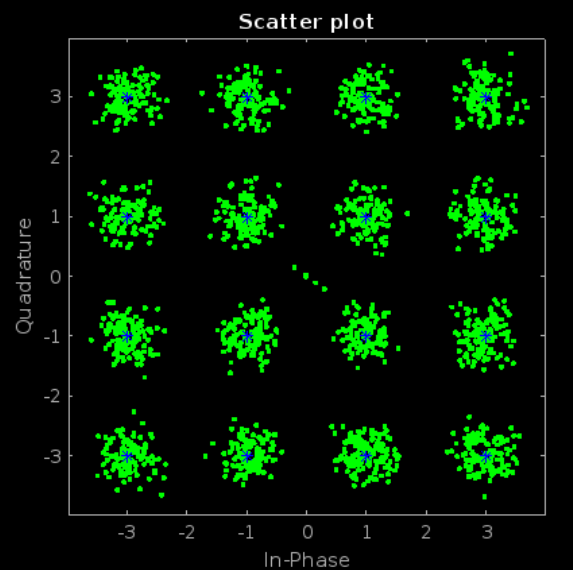
\includegraphics[width=0.45\textwidth]{img/matlab/qam.PNG}
	\caption{Constelación 16-QAM}
	\label{fig:qam}
\end{figure}
    
\vspace{3mm}

En este caso, se han decidido ajustar las tablas Q e I para establecer una codificación Gray. Esta se trata de una técnica específica que garantiza que solo un bit cambie entre dos valores consecutivos. Además, consigue minimizar la posibilidad de errores producidos por cambios de múltiples bits en la transmisión. A continuación, se puede visualizar la definición de cada una de las tablas:

\vspace{5mm}

\begin{lstlisting}[language=VHDL, style=mystyle, caption={Definición de la tabla de mapeado Q}]
type Array3Bit is array (0 to 15) of STD_LOGIC_VECTOR(2 downto 0);
constant tabla_mapeado_Q: Array3Bit :=
		("000", "001", "011", "010", 
		"110", "111", "101", "100",
		"000", "001", "011", "010", 
		"110", "111", "101", "100");
\end{lstlisting}

\pagebreak

\begin{lstlisting}[language=VHDL, style=mystyle, caption={Definición de la tabla de mapeado I}]
type Array3Bit is array (0 to 15) of STD_LOGIC_VECTOR(2 downto 0);
constant tabla_mapeado_I: Array3Bit := 
	("000", "000", "001", "001", 
	"011", "011", "010", "010",
	"110", "110", "111", "111", 
	"101", "101", "100", "100");
\end{lstlisting}

\vspace{3mm}
		
Por tanto, para mapear cada 











\section{Zero Padding}
%para optimizar el sistema de comunicación: el zero-padding 1:32. El zero-padding consiste en agregar ceros a la señal original, extendiendo su duración en el dominio del tiempo. En este caso, se aplica una relación de 1:32, lo que significa que por cada 1 bit de información transmitido, se añaden 31 bits de valor cero.

%La razón principal de aplicar zero-padding radica en la necesidad de preparar la señal para el filtrado pulse shaping del "root raised cosine" (RRC). El RRC es un tipo de filtro que se utiliza en sistemas de comunicación para dar forma a los pulsos transmitidos, minimizando la interferencia entre símbolos adyacentes. Este filtrado es crucial para cumplir con las restricciones espectrales y maximizar la eficiencia del espectro.

%El zero-padding aquí implementado garantiza que la señal de entrada al filtro RRC tenga una duración suficiente para lograr una respuesta de frecuencia óptima. Al incorporar este paso, se mejora la capacidad del sistema para recuperar la información transmitida con precisión y minimizar la interferencia intersimbólica.

%En resumen, este bloque desempeña un papel integral en la cadena de transmisión al combinar el mapeado de 16 QAM con el zero-padding 1:32, preparando así la señal para el posterior filtrado RRC. Esta estrategia contribuye significativamente a la mejora del rendimiento global del sistema de comunicación al garantizar una transmisión de datos confiable y eficiente en términos espectrales.

\section{Bloque de filtrado pulse shaping - RRC}



%193 coeficientes
%tenemos una ventana de 193 datos -> reg de desplazamiento (el actual+192 datos)
% y_filtro[t0] = sum193(y[ti]*coef[i])
%a la entrada hay valores enteros con signo(+1,-3,+3,-3)

%a=sfi(rrcfilter(1),16,16) %valor, nbits, nbits decimales)
%en este caso como los valores son de 0 con algo se ponen 16b decimales
%el error de precision es 2e-15/2 <- (1/2e-16)/2

%qr=sfi(rrcFilter',16)
%qr*2e17

%en freq response (en configuracion de vivado) coger gráfica
%config del filtro:
%se pone full precision 24, 3 bits signed

\vspace{3mm}

    \begin{figure}[h]
    	\centering
    	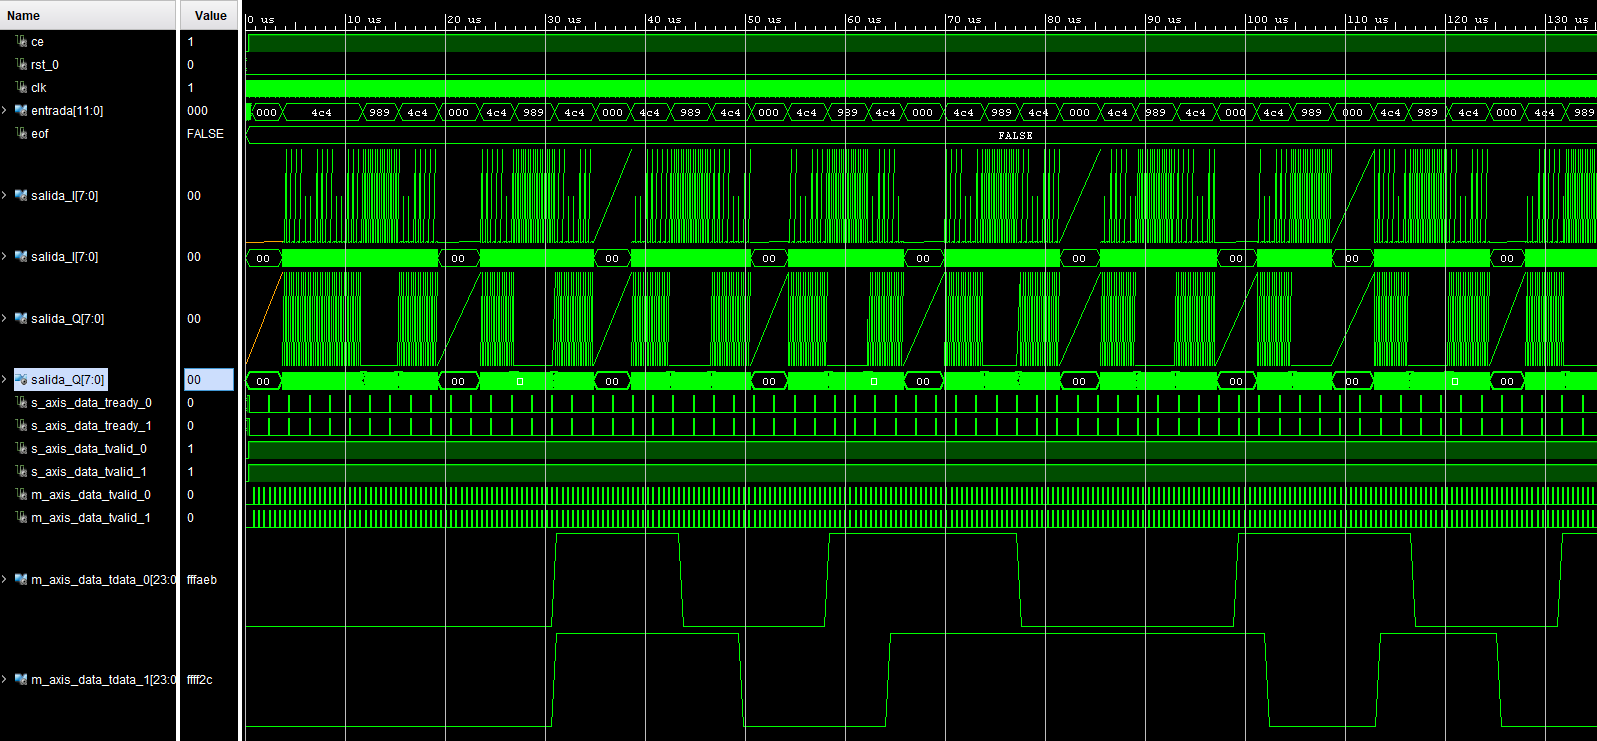
\includegraphics[width=1\textwidth]{img/matlab/rrc.PNG}
    	\caption{}
    	\label{fig:rrc}
    \end{figure}
    
\vspace{3mm}



